\documentclass[12pt]{article}

\usepackage[utf8]{inputenc}
\usepackage[T1]{fontenc}
\usepackage[spanish]{babel}
\usepackage[margin=2.3cm]{geometry}
\usepackage{setspace}
\onehalfspacing
\usepackage[sfdefault]{carlito}
\usepackage{graphicx}
\usepackage{booktabs}
\usepackage{hyperref}
\usepackage{listings}
\usepackage{xcolor}
\usepackage{enumitem}
\usepackage{float}
\usepackage{array}

\hypersetup{colorlinks=true, linkcolor=blue, urlcolor=blue, citecolor=blue}

\newcommand{\Universidad}{Universidad Internacional de La Rioja (UNIR)}
\newcommand{\Asignatura}{Sistemas Multiagente y Percepción Computacional}

\definecolor{codebg}{RGB}{248,248,248}
\definecolor{codecomment}{RGB}{0,102,51}
\definecolor{codekeyword}{RGB}{0,51,153}
\definecolor{codestring}{RGB}{153,0,0}

\lstdefinestyle{javaStyle}{
  language=Java,
  basicstyle=\ttfamily\small,
  backgroundcolor=\color{codebg},
  commentstyle=\color{codecomment},
  keywordstyle=\color{codekeyword}\bfseries,
  stringstyle=\color{codestring},
  numbers=left,
  numberstyle=\tiny,
  stepnumber=1,
  breaklines=true,
  frame=single,
  tabsize=4,
  showstringspaces=false
}

\title{\textbf{Actividad JADE con ejercicio adicional de comunicación entre agentes}}
\author{Sergio Andrés Majé Franco}
\date{\Asignatura \\ \Universidad \\ \today}

\begin{document}

\maketitle
\tableofcontents
\newpage

\section{Introducción}
La actividad se ha resuelto mediante un proyecto Java con JADE que no se limita a instalar la plataforma, sino que construye una demostración funcional de comunicación entre agentes. La solución implementa un cliente con interfaz gráfica Swing y un agente respondedor que procesa peticiones del usuario mediante mensajes ACL. De esta forma, la entrega muestra tanto la puesta en marcha del entorno como un caso práctico de interacción dentro de un sistema multiagente.

El enfoque elegido busca que la práctica sea presentable como trabajo de informática: el repositorio contiene código fuente, configuración reproducible con Maven, pruebas automáticas y una memoria técnica que describe la arquitectura y el comportamiento del sistema. La parte más relevante desde el punto de vista de la asignatura es que los agentes tienen responsabilidades diferenciadas y cooperan mediante intercambio de mensajes, que es uno de los mecanismos centrales del modelo de JADE.

\section{Entorno de trabajo e instalación}
\subsection{Tecnologías empleadas}
La solución se apoya en los siguientes elementos:

\begin{itemize}[leftmargin=*]
  \item Java 8 como nivel de compilación compatible con JADE.
  \item Maven como herramienta de construcción del proyecto.
  \item JADE como plataforma para la gestión del contenedor principal, el ciclo de vida de los agentes y el intercambio de mensajes.
  \item Swing para la interfaz gráfica del agente cliente.
\end{itemize}

\subsection{Integración de JADE}
La documentación oficial actual de JADE permite integrar la librería directamente desde Maven mediante JitPack \cite{jade-download}. Esta vía se ha elegido porque simplifica la preparación del entorno y deja el proyecto listo para compilar en cualquier equipo que disponga de Java y Maven.

\begin{lstlisting}[style=javaStyle, caption={Configuración esencial del proyecto Maven para usar JADE.}]
<repositories>
  <repository>
    <id>jitpack.io</id>
    <url>https://jitpack.io</url>
  </repository>
</repositories>

<dependency>
  <groupId>com.gitlab.jade-project</groupId>
  <artifactId>jade</artifactId>
  <version>master-SNAPSHOT</version>
</dependency>
\end{lstlisting}

\subsection{Observación sobre el procedimiento clásico}
El material de la actividad menciona el despliegue clásico mediante descargas manuales. Esa opción sigue siendo válida, pero en este trabajo se ha optado por la integración con Maven porque reduce errores de configuración, evita copiar librerías al proyecto y permite dejar un proceso de construcción más limpio. JADE continúa siendo una plataforma Java y los requisitos indicados por su documentación oficial son compatibles con la versión utilizada en esta práctica \cite{jade-start,jade-about}.

\section{Descripción general del proyecto}
\subsection{Estructura del repositorio}
El repositorio se divide en dos carpetas principales:

\begin{itemize}[leftmargin=*]
  \item \texttt{java/}: contiene el proyecto Maven, las clases de los agentes y las pruebas unitarias.
  \item \texttt{docs/}: contiene la memoria, la bibliografía, las capturas y los ficheros auxiliares para generar el documento final.
\end{itemize}

Esta separación permite mantener aislado el código ejecutable de la documentación y facilita la revisión de la entrega.

\subsection{Objetivo técnico del ejercicio adicional}
El ejercicio desarrollado consiste en un chat mínimo entre agentes. El usuario interactúa con una ventana Swing asociada al agente cliente y escribe órdenes o mensajes libres. El agente cliente transforma esa entrada en mensajes ACL dirigidos al agente respondedor. El agente respondedor interpreta la petición y devuelve una respuesta informativa. Finalmente, el agente cliente recibe la respuesta y la muestra en la transcripción de la interfaz.

Aunque se trata de una demostración pequeña, incluye varios elementos representativos de un sistema multiagente:

\begin{itemize}[leftmargin=*]
  \item existencia de múltiples agentes con identidad propia;
  \item comunicación asíncrona mediante mensajes ACL;
  \item separación de responsabilidades entre agentes;
  \item ejecución coordinada dentro de un contenedor principal de JADE.
\end{itemize}

\section{Arquitectura multiagente}
\subsection{Agentes implementados}
La solución incluye dos agentes y un punto de arranque:

\begin{itemize}[leftmargin=*]
  \item \texttt{Main}: crea el contenedor principal de JADE, configura el perfil de ejecución y arranca los agentes.
  \item \texttt{ChatClientAgent}: agente cliente que gestiona la interacción con el usuario.
  \item \texttt{ChatResponderAgent}: agente respondedor que procesa el contenido recibido y genera la contestación.
\end{itemize}

\subsection{Tipo de agente cliente}
El \texttt{ChatClientAgent} puede describirse como un agente de interfaz e intermediación. No realiza cálculos sobre el dominio ni toma decisiones complejas; su función principal es actuar como puente entre el usuario humano y la plataforma JADE. Este agente:

\begin{itemize}[leftmargin=*]
  \item crea o coordina la ventana Swing cuando la aplicación se ejecuta en modo interactivo;
  \item recoge la entrada textual del usuario;
  \item encola los mensajes para no bloquear la interfaz;
  \item envía solicitudes ACL al agente respondedor;
  \item recibe las respuestas y las presenta en la transcripción del chat.
\end{itemize}

Desde un punto de vista conceptual, es un agente orientado a la interacción humano-sistema. Su comportamiento es cíclico, reactivo a la llegada de mensajes y además coordinador de eventos procedentes de la interfaz gráfica.

\subsection{Tipo de agente respondedor}
El \texttt{ChatResponderAgent} puede clasificarse como un agente reactivo de servicio. No mantiene un modelo deliberativo complejo ni planifica a largo plazo; su papel es esperar mensajes, interpretar su contenido y producir una respuesta inmediata. En concreto:

\begin{itemize}[leftmargin=*]
  \item permanece a la espera de mensajes ACL entrantes;
  \item delega el procesamiento en \texttt{ResponderCommandProcessor};
  \item envía una respuesta al emisor original mediante \texttt{createReply()};
  \item registra por consola el mensaje recibido y la respuesta emitida.
\end{itemize}

Se trata de un agente adecuado para una primera práctica porque permite mostrar percepción del entorno de mensajes y reacción ante eventos sin introducir una lógica demasiado extensa.

\subsection{Flujo de comunicación}
La interacción principal del sistema sigue el siguiente recorrido:

\begin{enumerate}[leftmargin=*]
  \item el usuario escribe un texto en la ventana Swing;
  \item el \texttt{ChatClientAgent} lo encapsula en un mensaje ACL de tipo \texttt{REQUEST};
  \item el \texttt{ChatResponderAgent} recibe la petición;
  \item el respondedor analiza el contenido y construye una respuesta;
  \item el respondedor devuelve un mensaje ACL de tipo \texttt{INFORM};
  \item el cliente recibe la contestación y la representa en pantalla.
\end{enumerate}

Este patrón es útil académicamente porque muestra un intercambio completo solicitud-respuesta entre agentes locales dentro de un mismo contenedor JADE.

\begin{figure}[htbp]
\centering
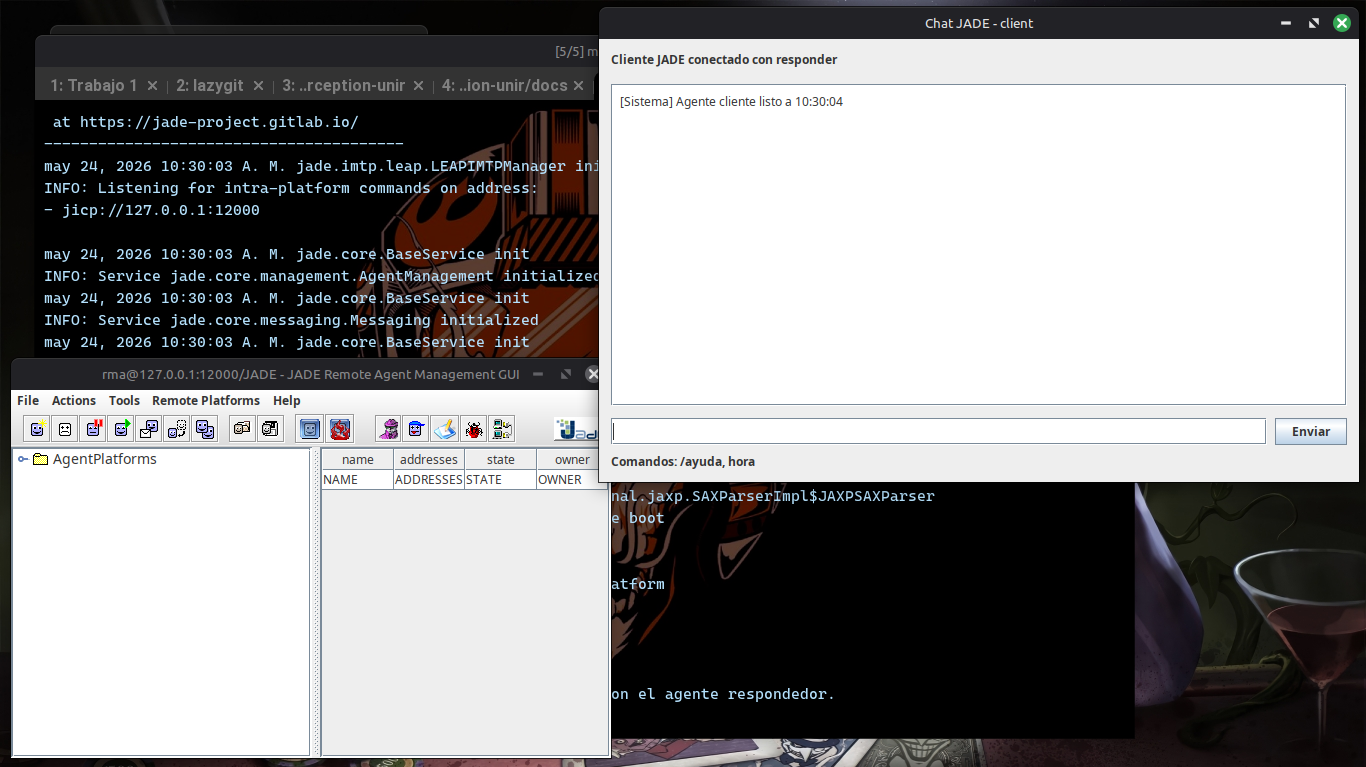
\includegraphics[width=\textwidth]{captures/capture-01.png}
\caption{Arranque del contenedor principal de JADE, consola administrativa y ventana del agente cliente.}
\end{figure}

\section{Comportamiento funcional del sistema}
\subsection{Interfaz del agente cliente}
La interfaz gráfica está implementada en la clase \texttt{ChatWindow}. La ventana incluye un área de transcripción, un campo de texto para introducir mensajes, un botón de envío y una línea de ayuda con los comandos disponibles. Esta interfaz no contiene lógica JADE directa; únicamente reenvía la entrada del usuario al agente cliente. Esta separación es una decisión correcta de diseño porque evita mezclar la presentación con la mensajería.

\begin{figure}[htbp]
\centering
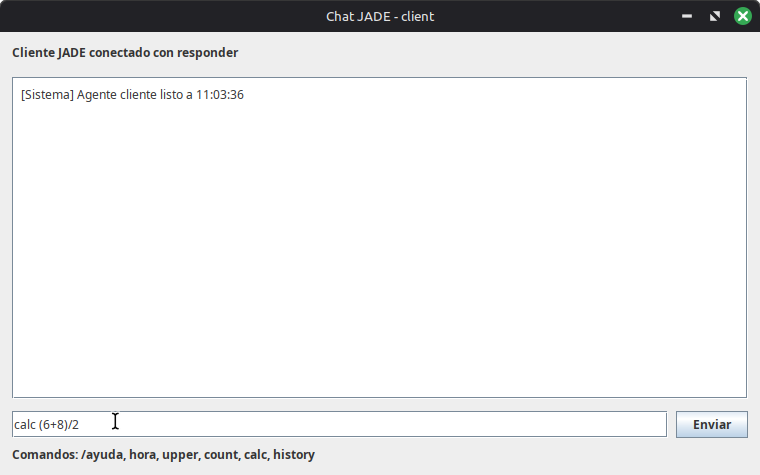
\includegraphics[width=0.82\textwidth]{captures/capture-02.png}
\caption{Ventana del agente cliente con la orden \texttt{calc (6+8)/2} preparada para su envío.}
\end{figure}

\subsection{Comandos soportados por el agente respondedor}
El comportamiento del respondedor ya no se reduce a un eco simple. La lógica de comandos se concentra en un procesador específico desacoplado de JADE, lo que facilita explicar y probar el comportamiento real del agente. Los comandos disponibles son los siguientes:

\begin{itemize}[leftmargin=*]
  \item \texttt{hora} o \texttt{/hora}: devuelve la hora actual del sistema.
  \item \texttt{ayuda} o \texttt{/ayuda}: muestra la lista de comandos soportados.
  \item \texttt{upper <texto>}: transforma el texto recibido a mayúsculas.
  \item \texttt{count <texto>}: informa del número de palabras y caracteres.
  \item \texttt{calc <expresion>}: evalúa una expresión aritmética simple con operadores básicos y paréntesis.
  \item \texttt{history}: devuelve el historial reciente de mensajes procesados.
\end{itemize}

Si el texto no coincide con ninguno de los comandos anteriores, el agente responde con un eco del contenido recibido. Esto garantiza que siempre exista una contestación visible y facilita la comprobación manual del intercambio de mensajes.

\subsection{Valor académico del comportamiento implementado}
Aunque los comandos son sencillos, el ejercicio permite evidenciar varios conceptos relevantes:

\begin{itemize}[leftmargin=*]
  \item el agente respondedor no es una ventana estática, sino un componente autónomo que procesa solicitudes;
  \item la lógica de respuesta está desacoplada de la infraestructura JADE y puede probarse mediante tests unitarios;
  \item la conversación no depende de llamadas directas entre clases, sino de mensajería ACL;
  \item el uso de un historial muestra que el agente mantiene un pequeño estado interno.
\end{itemize}

\begin{figure}[htbp]
\centering
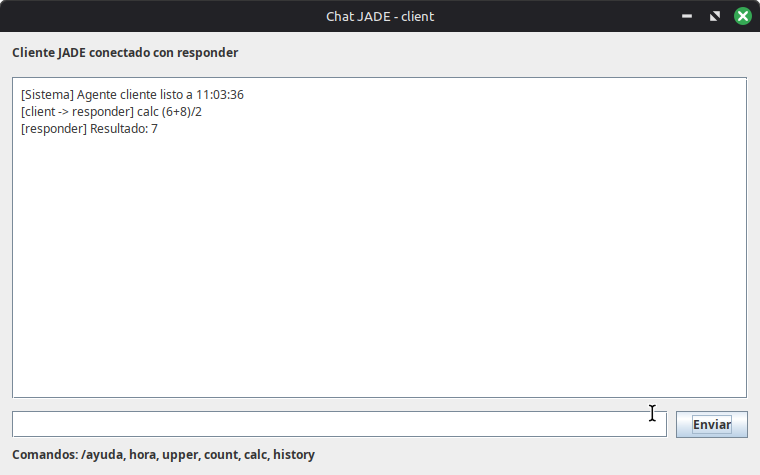
\includegraphics[width=0.82\textwidth]{captures/capture-03.png}
\caption{Resultado visible en la interfaz tras enviar la operación \texttt{calc (6+8)/2}.}
\end{figure}

\section{Puesta en marcha}
La ejecución interactiva del proyecto se realiza desde la carpeta \texttt{java/}:

\begin{lstlisting}[style=javaStyle, caption={Comando de ejecución del ejercicio en modo gráfico.}]
cd java
mvn exec:java -Dexec.mainClass=com.unir.jade.chat.Main
\end{lstlisting}

Además, el proyecto incluye un modo demostración activable con el argumento \texttt{--demo}. Este modo es útil para verificar el comportamiento en entornos sin interfaz gráfica, ya que envía automáticamente una secuencia predefinida de mensajes y cierra la plataforma al finalizar.

\section{Pruebas y validación}
\subsection{Pruebas automáticas}
El proyecto incorpora pruebas unitarias sobre dos piezas que concentran lógica reutilizable:

\begin{itemize}[leftmargin=*]
  \item \texttt{ChatTranscriptFormatterTest}, para verificar el formato de las líneas mostradas en la transcripción.
  \item \texttt{ResponderCommandProcessorTest}, para comprobar eco, mayúsculas, conteo, cálculo, gestión de expresiones erróneas e historial.
\end{itemize}

Este enfoque es importante porque la parte más fácil de verificar de forma automática no es la interfaz gráfica, sino la lógica de transformación y respuesta.

\lstinputlisting[style=javaStyle, caption={Pruebas del procesador de comandos del agente respondedor.}]{../java/src/test/java/com/unir/jade/chat/ResponderCommandProcessorTest.java}

\subsection{Evidencia de ejecución}
La salida de consola del modo demostración confirma el ciclo completo de comunicación entre agentes: arranque de la plataforma, envío de mensajes del cliente, recepción por parte del respondedor y devolución de la respuesta.

\lstinputlisting[basicstyle=\ttfamily\small, backgroundcolor=\color{codebg}, frame=single, breaklines=true, caption={Salida de ejemplo del modo demostración.}]{sample-output.txt}

\subsection{Comprobaciones realizadas}
La validación de la práctica se ha apoyado en cuatro comprobaciones:

\begin{itemize}[leftmargin=*]
  \item compilación correcta del proyecto Maven;
  \item ejecución satisfactoria de las pruebas unitarias;
  \item arranque del contenedor principal de JADE y de los dos agentes;
  \item verificación manual de la interacción desde la interfaz Swing.
\end{itemize}

\section{Conclusiones}
La práctica queda resuelta con una entrega más sólida que una simple instalación de JADE, ya que presenta un caso funcional de comunicación entre agentes con interfaz gráfica y lógica de respuesta propia. El sistema demuestra que JADE puede emplearse para construir aplicaciones donde varios agentes cooperan mediante mensajes y mantienen responsabilidades bien separadas.

Desde la perspectiva de la asignatura, el agente cliente puede entenderse como un agente de interfaz e intermediación, mientras que el agente respondedor actúa como un agente reactivo de servicio. Esta distinción aporta valor al trabajo porque no solo enseña a arrancar la plataforma, sino también a diseñar roles diferentes dentro de una arquitectura multiagente sencilla pero coherente.

\bibliographystyle{plain}
\bibliography{bib/references}

\end{document}
